\documentclass[aspectratio=169, 10pt]{beamer}

% Encoding and Typography
\usepackage[utf8]{inputenc}
\usepackage[T1]{fontenc}
\usepackage{FiraSans}
\usepackage{microtype}
\usepackage{amsmath}

% Graphics and Layout
\usepackage{graphicx}
\usepackage{tikz}
\usetikzlibrary{calc,positioning,shapes,arrows.meta}
\usepackage{tcolorbox}
\tcbuselibrary{skins,raster}
\usepackage{tabularx}
\usepackage{booktabs}
\usepackage{xcolor}
\usepackage{appendixnumberbeamer}

% =========================================================================
% COLOR PALETTE (Strict Monochrome + Single Muted Emerald Accent)
% =========================================================================
\definecolor{bgdark}{HTML}{0F172A}       % Deep Slate (#0F172A)
\definecolor{cardsurface}{HTML}{1E293B}  % Uniform Elevated Slate (#1E293B)
\definecolor{cardborder}{HTML}{334155}   % Uniform Subtle Gray (#334155)
\definecolor{cardinner}{HTML}{141D2E}    % Inner Container
\definecolor{textwhite}{HTML}{F8FAFC}    % Pure White (#F8FAFC)
\definecolor{textmuted}{HTML}{CBD5E1}    % Light Gray (#CBD5E1)
\definecolor{textdim}{HTML}{94A3B8}      % Dim Slate Gray

% Single Accent: Used ONLY for section pill, 2 stat numbers, and highlights
\definecolor{accentemerald}{HTML}{10B981}% Muted Emerald (#10B981)

% =========================================================================
% BEAMER SETTINGS
% =========================================================================
\setbeamersize{text margin left=12mm, text margin right=12mm}
\setbeamercolor{background canvas}{bg=bgdark}
\setbeamercolor{normal text}{fg=textwhite}
\setbeamertemplate{navigation symbols}{}

% Standard Clean Bullets
\setbeamertemplate{itemize items}{\scriptsize\textcolor{textdim}{\textbullet}}
\setbeamertemplate{itemize subitem}{\tiny\textcolor{textdim}{\textbullet}}

\newenvironment{compactlist}{%
  \begin{itemize}%
    \setlength{\itemsep}{1.5pt}%
    \setlength{\topsep}{0pt}%
    \setlength{\partopsep}{0pt}%
    \setlength{\parsep}{0pt}%
    \setlength{\parskip}{0pt}%
}{\end{itemize}}

% Sleek 1-Line Clean Footer
\setbeamertemplate{footline}{
  \begin{beamercolorbox}[wd=\paperwidth,ht=4.5mm,dp=2.5mm,leftskip=12mm,rightskip=12mm]{}
    \tiny\textcolor{textdim}{\textbf{Sample Browser} \quad \textbar \quad FAF.PCAS25.1 · Midterm 1}
    \hfill
    \tiny\textcolor{textdim}{Technical University of Moldova (FCIM)}
    \hfill
    \tiny\textcolor{textwhite}{\textbf{\insertframenumber}} \textcolor{textdim}{/} \textcolor{textdim}{\inserttotalframenumber}
  \end{beamercolorbox}
}

% =========================================================================
% TCOLORBOX STYLES (Strict uniform border & padding)
% =========================================================================
\tcbset{
  standardcard/.style={
    enhanced,
    colback=cardsurface,
    colframe=cardborder,
    coltext=textwhite,
    boxrule=0.6pt,
    arc=3pt,
    left=8pt, right=8pt, top=6pt, bottom=6pt,
    boxsep=0pt
  },
  innercard/.style={
    enhanced,
    colback=cardinner,
    colframe=cardborder,
    coltext=textwhite,
    boxrule=0.5pt,
    arc=2.5pt,
    left=7pt, right=7pt, top=5pt, bottom=5pt,
    boxsep=0pt
  }
}

% Slide Header Macro: #1: Category Tag, #2: Slide Title
% Top margin: clear space above section pill
\newcommand{\slideheader}[2]{%
  \vspace*{2mm}%
  \noindent\begin{minipage}{\textwidth}%
    \begin{tikzpicture}[baseline=(pill.base)]%
      \node[fill=cardsurface, draw=cardborder, line width=0.6pt, rounded corners=2pt, inner sep=2.5pt] (pill) {%
        \tiny\bfseries\textcolor{accentemerald}{#1}%
      };%
    \end{tikzpicture}\\[1.6mm]%
    {\large\bfseries\textcolor{textwhite}{#2}}%
  \end{minipage}\par\vspace{2.5mm}%
}

% =========================================================================
% PRESENTATION SLIDES (9 Core Slides + 1 Optional Appendix Slide)
% =========================================================================
\begin{document}

\begin{frame}[t]
  \vspace*{2mm}
  % Top Header Row
  \noindent\begin{minipage}{\textwidth}
    
\begin{tikzpicture}[baseline=(pill.base)]
      \node[fill=cardsurface, draw=cardborder, line width=0.6pt, rounded corners=2.5pt, inner sep=2.5pt] (pill) {
        \tiny\bfseries\textcolor{textwhite}{TECHNICAL UNIVERSITY OF MOLDOVA · FCIM · FAF.PCAS25.1}
      };
    \end{tikzpicture}%
    \hfill%
    
\begin{tikzpicture}[baseline=(pill2.base)]
      \node[fill=cardsurface, draw=cardborder, line width=0.6pt, rounded corners=2.5pt, inner sep=2.5pt] (pill2) {
        \tiny\bfseries\textcolor{accentemerald}{MIDTERM 1 DEFENSE · 7-MIN PITCH}
      };
    \end{tikzpicture}
  \end{minipage}

  \vspace{3mm}

  % Main Title Hero Card
  \begin{tcolorbox}[standardcard, left=9pt, right=9pt, top=8pt, bottom=8pt]
    \begin{columns}[onlytextwidth, c]
      \begin{column}{0.75\textwidth}
        {\LARGE\bfseries\textcolor{textwhite}{Better Spotify / \textcolor{accentemerald}{Sample Browser}}}\par\vspace{1.5mm}
        {\normalsize\textcolor{textmuted}{Granular Audio Passage Discovery for Independent Music Producers}}\par\vspace{2mm}
        {\scriptsize\textcolor{textdim}{Problem-Based Learning Journey: Evolving from a Passive Playback Concept into an Active Creator Workspace}}
      \end{column}
      \begin{column}{0.22\textwidth}
        \centering
        \begin{tcolorbox}[enhanced, colback=white, colframe=cardborder, arc=3pt, boxrule=0.6pt, left=2mm, right=2mm, top=2mm, bottom=2mm, halign=center]
          
\includegraphics[width=\linewidth, height=1.05cm, keepaspectratio]{images/UTM_Logo.png}
        \end{tcolorbox}
      \end{column}
    \end{columns}
  \end{tcolorbox}

  \vspace{3mm}

  % Bottom Metadata Row
  \begin{columns}[onlytextwidth, T]
    % Students Card
    \begin{column}{0.485\textwidth}
      \begin{tcolorbox}[standardcard, top=5pt, bottom=5pt]
        {\scriptsize\bfseries\textcolor{textwhite}{TEAM 16 (FAF STUDENTS)}}\par\vspace{1.5mm}
        \begin{tabularx}{\textwidth}{@{}l X l X@{}}
          \tiny\textcolor{textmuted}{Bogdan Glavan} & \tiny\textcolor{textdim}{FAF-261} &
          \tiny\textcolor{textmuted}{Leonid Tiscenco} & \tiny\textcolor{textdim}{FAF-263} \\
          \tiny\textcolor{textmuted}{Andrei Simon} & \tiny\textcolor{textdim}{FAF-261} &
          \tiny\textcolor{textmuted}{Mihai-Constantin Sîrghii} & \tiny\textcolor{textdim}{FAF-262} \\
          \tiny\textcolor{textmuted}{Nikita Creciun} & \tiny\textcolor{textdim}{FAF-263} &
          & \\
        \end{tabularx}
      \end{tcolorbox}
    \end{column}

    % Mentor & Course Card
    \begin{column}{0.485\textwidth}
      \begin{tcolorbox}[standardcard, top=5pt, bottom=5pt]
        {\scriptsize\bfseries\textcolor{textwhite}{PROJECT SUPERVISION}}\par\vspace{1.5mm}
        {\tiny\textbf{\textcolor{textwhite}{Mentor:}} \textcolor{textmuted}{Elena Graur}}\par\vspace{0.8mm}
        {\tiny\textcolor{textmuted}{Faculty of Computers, Informatics and Microelectronics (FCIM)}}\par\vspace{0.5mm}
        {\tiny\textcolor{textdim}{Department of Software Engineering and Automatics · Chişinău, 2026}}
      \end{tcolorbox}
    \end{column}
  \end{columns}
\end{frame}

\begin{frame}[t]
  \slideheader{01. INTRODUCTION \& CONTEXT}{The Environment and Reality of Audio Sampling}

  \begin{columns}[onlytextwidth, c]
    % Left Column: Prominent Studio Photograph
    \begin{column}{0.48\textwidth}
      \begin{tcolorbox}[standardcard, top=3pt, bottom=3pt]
        \centering
        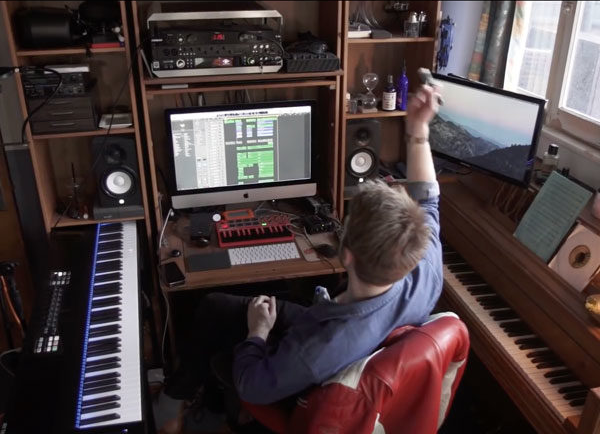
\includegraphics[width=\linewidth, height=4.2cm, keepaspectratio]{images/musician_cropped.png}\par\vspace{1mm}
        {\tiny\textcolor{textdim}{\textbf{Production Context:} Bedroom workstation with DAW, keyboard, and monitoring.}}
      \end{tcolorbox}
    \end{column}

    % Right Column: Definition & Two Key Metrics
    \begin{column}{0.49\textwidth}
      % Definition Card
      \begin{tcolorbox}[standardcard, top=8pt, bottom=8pt, left=8pt, right=8pt]
        {\tiny\bfseries\textcolor{accentemerald}{CORE CONCEPT}}\par\vspace{1.5mm}
        {\normalsize\bfseries\textcolor{textwhite}{Sampling: Reusing a portion of an existing recording in a new composition.}}\par\vspace{2mm}
        {\scriptsize\textcolor{textmuted}{Producers hunt for localized \textbf{2--8 bar passages} (4--30s), not whole songs.}}
      \end{tcolorbox}

      \vspace{3mm}

      % Two Key Numbers
      \begin{columns}[onlytextwidth, T]
        \begin{column}{0.48\textwidth}
          \begin{tcolorbox}[innercard, top=6pt, bottom=6pt]
            \centering
            {\LARGE\bfseries\textcolor{accentemerald}{17\%}}\par\vspace{0.8mm}
            {\scriptsize\bfseries\textcolor{textwhite}{Billboard Hot 100}}\par\vspace{0.4mm}
            {\tiny\textcolor{textdim}{Hits rely on samples (Tracklib)}}
          \end{tcolorbox}
        \end{column}
        \begin{column}{0.48\textwidth}
          \begin{tcolorbox}[innercard, top=6pt, bottom=6pt]
            \centering
            {\LARGE\bfseries\textcolor{accentemerald}{250M+}}\par\vspace{0.8mm}
            {\scriptsize\bfseries\textcolor{textwhite}{Streaming Catalog}}\par\vspace{0.4mm}
            {\tiny\textcolor{textdim}{Tracks indexed mainly at track level}}
          \end{tcolorbox}
        \end{column}
      \end{columns}
    \end{column}
  \end{columns}
\end{frame}

\begin{frame}[t]
  \slideheader{02. DOMAIN ANALYSIS \& EXISTING TOOLS}{Three Existing Paradigms vs. Passage Discovery}

  % Three Equal Visual Product Cards
  \begin{columns}[onlytextwidth, T]
    % Card 1: Splice
    \begin{column}{0.315\textwidth}
      \begin{tcolorbox}[standardcard, top=4pt, bottom=4pt]
        {\small\bfseries\textcolor{textwhite}{Splice}}\par\vspace{0.4mm}
        {\scriptsize\bfseries\textcolor{accentemerald}{Ready-Made Samples}}\par\vspace{1.2mm}
        \centering
        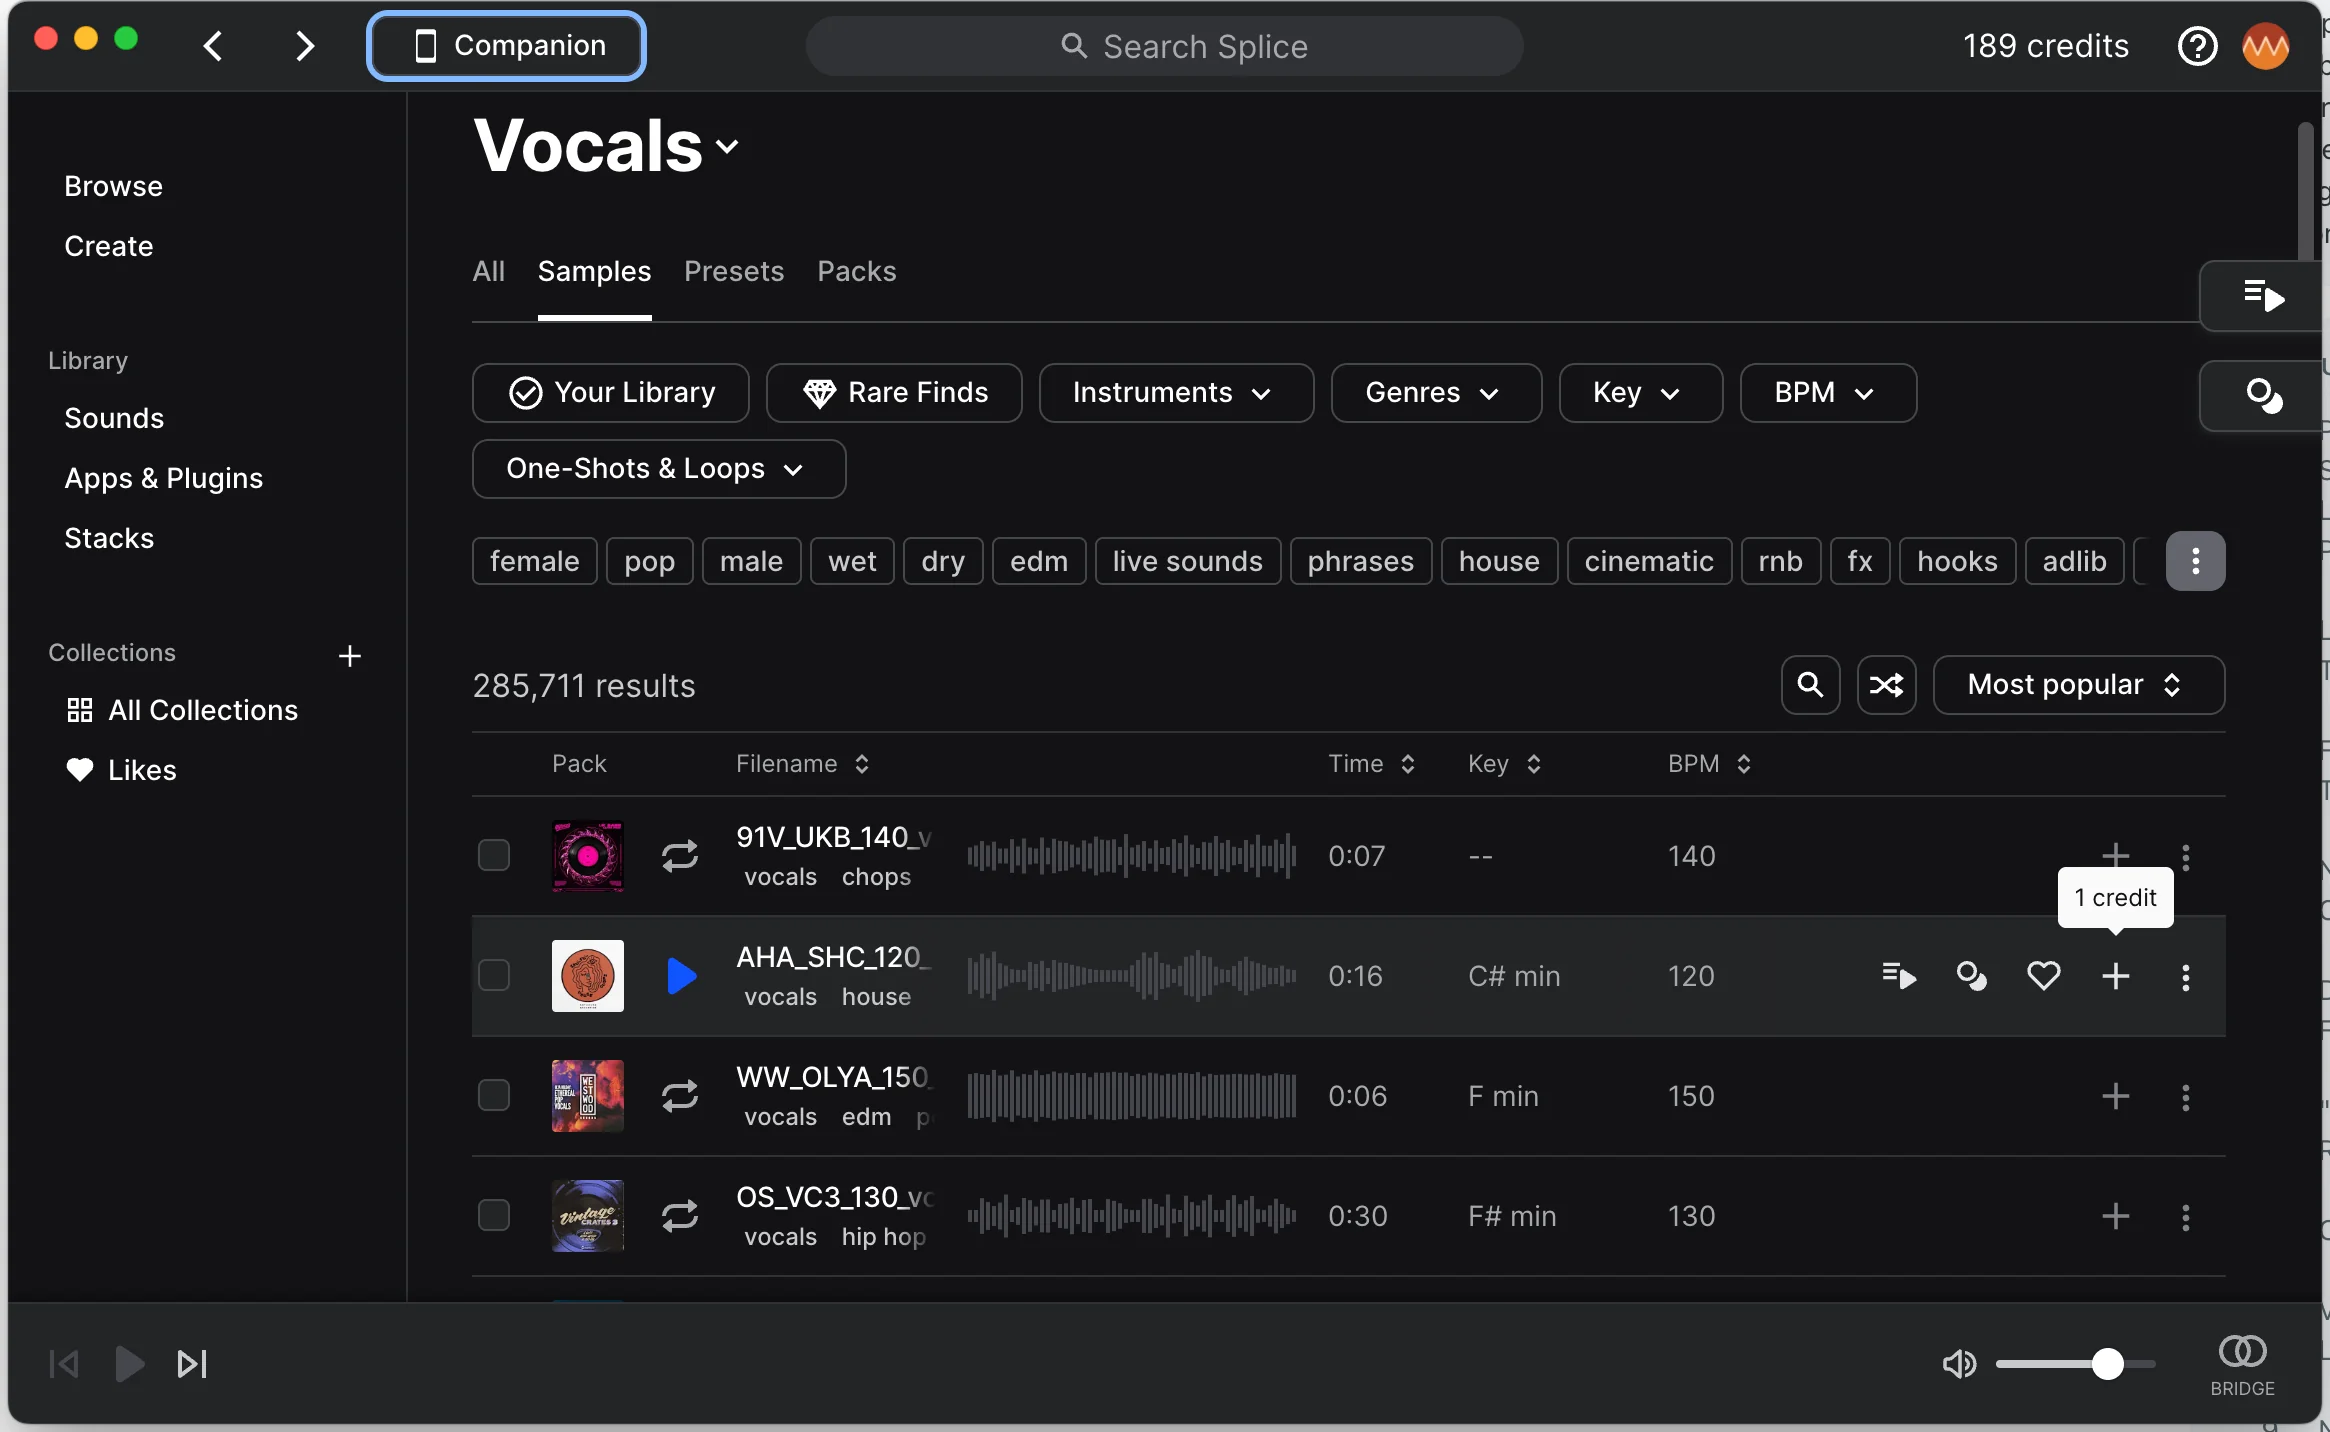
\includegraphics[width=\linewidth, height=2.25cm, keepaspectratio]{images/splice_workflow.png}\par\vspace{1.2mm}
        {\tiny\textcolor{textmuted}{Catalog of pre-cut loops \& one-shots; prepared library workflow.}}
      \end{tcolorbox}
    \end{column}

    % Card 2: Samplette.io
    \begin{column}{0.315\textwidth}
      \begin{tcolorbox}[standardcard, top=4pt, bottom=4pt]
        {\small\bfseries\textcolor{textwhite}{Samplette.io}}\par\vspace{0.4mm}
        {\scriptsize\bfseries\textcolor{accentemerald}{Discover Full Recordings}}\par\vspace{1.2mm}
        \centering
        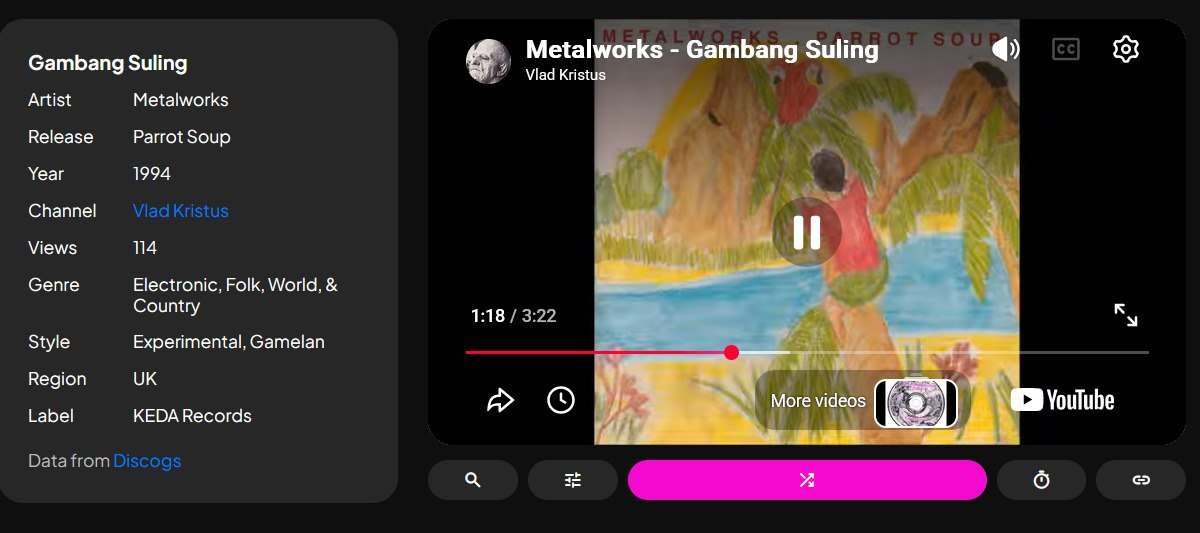
\includegraphics[width=\linewidth, height=2.25cm, keepaspectratio]{images/samplette_work.jpg}\par\vspace{1.2mm}
        {\tiny\textcolor{textmuted}{Randomized YouTube digging via Discogs; whole-track search only.}}
      \end{tcolorbox}
    \end{column}

    % Card 3: Tracklib
    \begin{column}{0.315\textwidth}
      \begin{tcolorbox}[standardcard, top=4pt, bottom=4pt]
        {\small\bfseries\textcolor{textwhite}{Tracklib}}\par\vspace{0.4mm}
        {\scriptsize\bfseries\textcolor{accentemerald}{Licensed Catalog + Tools}}\par\vspace{1.2mm}
        \centering
        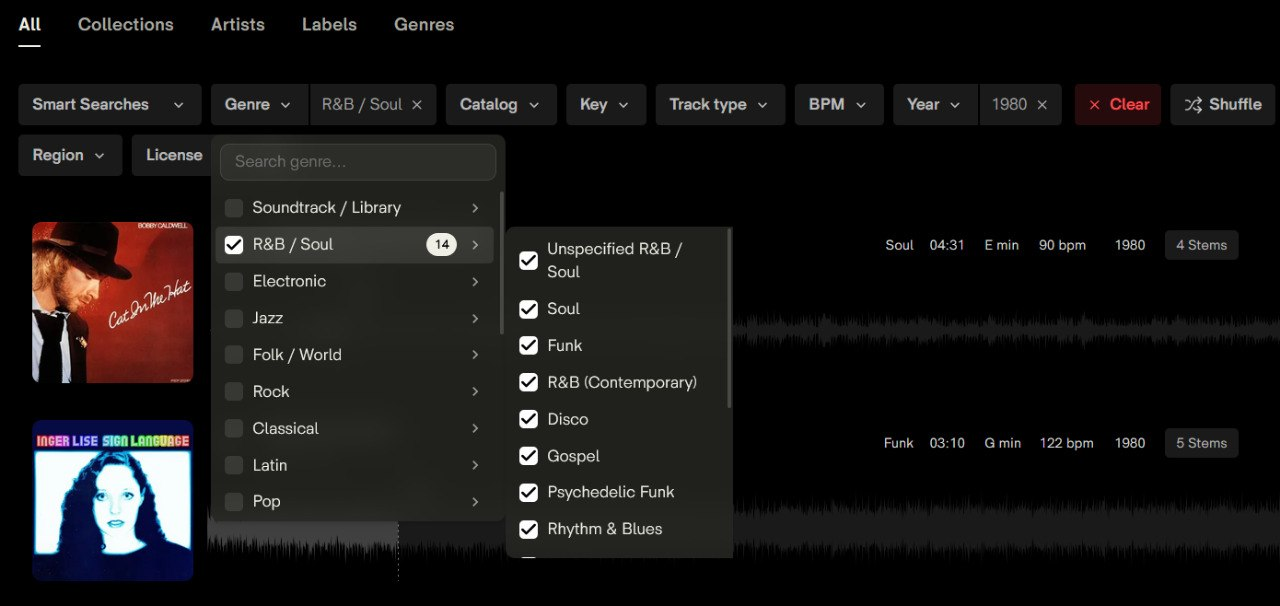
\includegraphics[width=\linewidth, height=2.25cm, keepaspectratio]{images/tracklib_search.jpg}\par\vspace{1.2mm}
        {\tiny\textcolor{textmuted}{Pre-cleared songs with stem isolation and bar-looping tools.}}
      \end{tcolorbox}
    \end{column}
  \end{columns}

  \vspace{2.5mm}

  % Bottom Unified Differentiator
  \begin{tcolorbox}[innercard, left=6pt, right=6pt, top=3.5pt, bottom=3.5pt]
    \centering
    {\small\textbf{\textcolor{accentemerald}{Sample Browser:}} \textcolor{textwhite}{Discover and compare passages across recordings.}}
  \end{tcolorbox}
\end{frame}
\begin{frame}[t]
  \slideheader{03. PROBLEM ANALYSIS \& PIVOT}{The Core Problem \& Strategic Workflow Pivot}

  % Central Statement Headline
  \begin{tcolorbox}[standardcard, top=2.5pt, bottom=2.5pt]
    \centering
    {\large\bfseries\textcolor{textwhite}{Producers lack an efficient way to find specific passages inside full recordings.}}\par\vspace{0.2mm}
    {\tiny\textcolor{textdim}{Streaming catalogs index music as 4-minute monoliths; producers search by sound timbre for 2--8 bar passages.}}
  \end{tcolorbox}

  \vspace{1mm}

  % Main Visual: Timeline Diagram of 4-min Recording vs. Short Passages
  \begin{tcolorbox}[innercard, top=2.5pt, bottom=2.5pt]
    \centering
    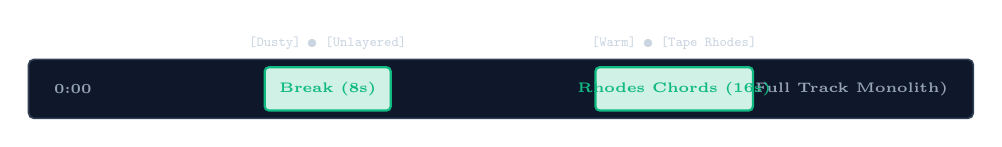
\begin{tikzpicture}[x=1cm, y=1cm]
      % Track bar background
      \draw[fill=bgdark, draw=cardborder, line width=0.6pt, rounded corners=2pt] (0,0) rectangle (12, 0.75);
      
      % Track labels
      \node[anchor=west, textdim, font=\tiny\bfseries] at (0.2, 0.375) {0:00};
      \node[anchor=east, textdim, font=\tiny\bfseries] at (11.8, 0.375) {4:00 (Full Track Monolith)};

      % Sub-track passage 1: Break
      \draw[fill=accentemerald!20, draw=accentemerald, line width=0.8pt, rounded corners=1.5pt] (3.0, 0.1) rectangle (4.6, 0.65);
      \node[font=\tiny\bfseries, text=accentemerald] at (3.8, 0.375) {Break (8s)};
      
      % Sub-track passage 2: Rhodes
      \draw[fill=accentemerald!20, draw=accentemerald, line width=0.8pt, rounded corners=1.5pt] (7.2, 0.1) rectangle (9.2, 0.65);
      \node[font=\tiny\bfseries, text=accentemerald] at (8.2, 0.375) {Rhodes Chords (16s)};

      % Acoustic vocabulary tags pointing
      \node[anchor=south, font=\tiny\bfseries, text=textmuted] at (3.8, 0.75) {\texttt{[Dusty]} \textbullet{} \texttt{[Unlayered]}};
      \node[anchor=south, font=\tiny\bfseries, text=textmuted] at (8.2, 0.75) {\texttt{[Warm]} \textbullet{} \texttt{[Tape Rhodes]}};
    \end{tikzpicture}
  \end{tcolorbox}

  \vspace{1mm}

  % Row: Workflow Comparison (Current vs. Proposed)
  \begin{columns}[onlytextwidth, T]
    % Current Workflow
    \begin{column}{0.485\textwidth}
      \begin{tcolorbox}[standardcard, top=2.5pt, bottom=2.5pt]
        {\scriptsize\bfseries\textcolor{textdim}{Current Scrubbing Loop:}}\par\vspace{0.6mm}
        \centering
        {\tiny\textbf{\textcolor{textmuted}{Full Track}} \textcolor{textdim}{$\longrightarrow$} \textbf{\textcolor{textmuted}{Manual Scrub}} \textcolor{textdim}{$\longrightarrow$} \textbf{\textcolor{cardborder!40!textwhite}{Repeat / Flow Lost}}}
      \end{tcolorbox}
    \end{column}

    % Proposed Workflow
    \begin{column}{0.485\textwidth}
      \begin{tcolorbox}[standardcard, top=2.5pt, bottom=2.5pt]
        {\scriptsize\bfseries\textcolor{accentemerald}{Proposed Passage Workflow:}}\par\vspace{0.6mm}
        \centering
        {\tiny\textbf{\textcolor{textwhite}{Describe Sound}} \textcolor{textdim}{$\longrightarrow$} \textbf{\textcolor{accentemerald}{Find Passage}} \textcolor{textdim}{$\longrightarrow$} \textbf{\textcolor{accentemerald}{Jump to Cue}}}
      \end{tcolorbox}
    \end{column}
  \end{columns}

  \vspace{1mm}

  % Strategic Pivot Strip
  \begin{tcolorbox}[innercard, left=6pt, right=6pt, top=2pt, bottom=2pt]
    \centering
    {\tiny\bfseries\textcolor{textdim}{PBL Strategic Pivot:}} \quad
    {\tiny\textcolor{textmuted}{Consumer streaming shell} \textcolor{textdim}{$\longrightarrow$} \textcolor{textmuted}{Spotify API locks (audio endpoints deprecated)} \textcolor{textdim}{$\longrightarrow$} \textbf{\textcolor{accentemerald}{Creator-focused passage search}}}
  \end{tcolorbox}
\end{frame}

\begin{frame}[t]
  \slideheader{04. TARGET GROUP \& USER PERSONAS}{Two Illustrative Creator Personas (Validation Planned)}

  \begin{columns}[onlytextwidth, T]
    % Persona A: Alex "Kaelo" Miller
    \begin{column}{0.485\textwidth}
      \begin{tcolorbox}[standardcard, top=8pt, bottom=8pt, left=7pt, right=7pt]
        \begin{columns}[onlytextwidth, c]
          % Portrait (Enlarged ~30%, Minimalist Vector Art)
          \begin{column}{0.38\textwidth}
            \centering
            \begin{tcolorbox}[enhanced, colback=cardinner, colframe=cardborder, boxrule=0.6pt, arc=3pt, left=1pt, right=1pt, top=1pt, bottom=1pt]
              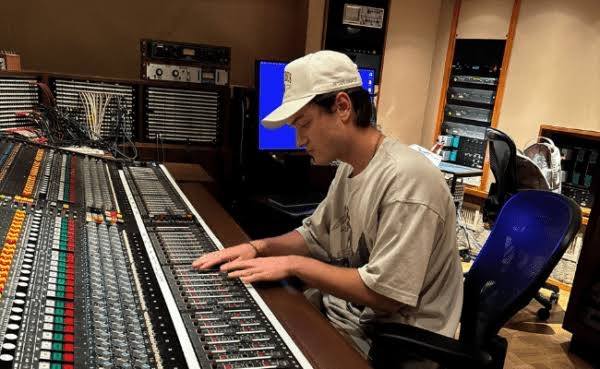
\includegraphics[width=\linewidth, height=2.8cm, keepaspectratio]{images/alex_photo.png}
            \end{tcolorbox}
          \end{column}

          % Details
          \begin{column}{0.58\textwidth}
            {\small\bfseries\textcolor{textwhite}{Alex Miller}}\\[0.2mm]
            {\tiny\bfseries\textcolor{accentemerald}{Aspiring Producer} \textcolor{textdim}{\textbar{} 22}}\par\vspace{1.5mm}
            
            {\tiny\textbullet{} \textbf{Role:} Bedroom producer (FL Studio)}\\[0.8mm]
            {\tiny\textbullet{} \textbf{Time:} 8--12 hrs/week creative time}\\[0.8mm]
            {\tiny\textbullet{} \textbf{Friction:} Scrubbing full-length tracks}\par\vspace{2mm}

            \begin{tcolorbox}[innercard, top=3pt, bottom=3pt, left=4pt, right=4pt]
              {\tiny\textcolor{textdim}{Scenario:}\\[0.2mm]
              \textbf{\textcolor{textwhite}{Found vocal}}\\[0.2mm]
              \textbf{\textcolor{accentemerald}{$\rightarrow$} \textcolor{textwhite}{needs matching guitar}}}
            \end{tcolorbox}
          \end{column}
        \end{columns}
      \end{tcolorbox}
    \end{column}

    % Persona B: Annie Lee
    \begin{column}{0.485\textwidth}
      \begin{tcolorbox}[standardcard, top=8pt, bottom=8pt, left=7pt, right=7pt]
        \begin{columns}[onlytextwidth, c]
          % Portrait (Enlarged ~30%, Minimalist Vector Art)
          \begin{column}{0.38\textwidth}
            \centering
            \begin{tcolorbox}[enhanced, colback=cardinner, colframe=cardborder, boxrule=0.6pt, arc=3pt, left=1pt, right=1pt, top=1pt, bottom=1pt]
              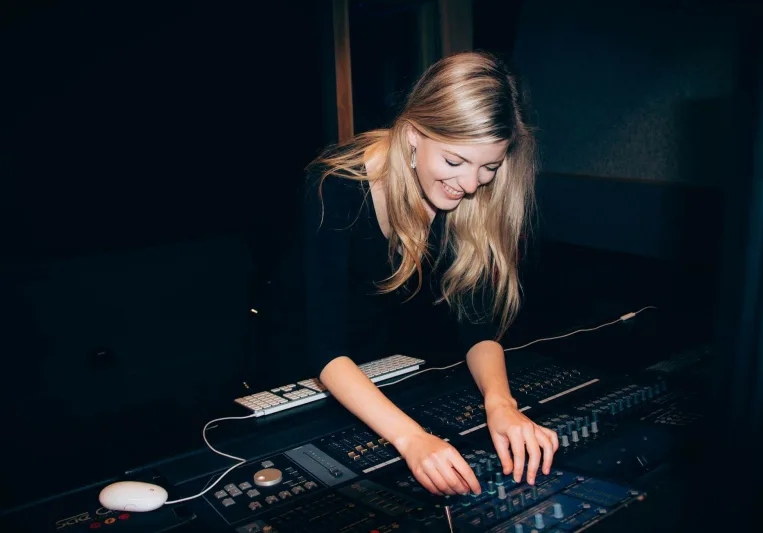
\includegraphics[width=\linewidth, height=2.8cm, keepaspectratio]{images/annie_photo.png}
            \end{tcolorbox}
          \end{column}

          % Details
          \begin{column}{0.58\textwidth}
            {\small\bfseries\textcolor{textwhite}{Annie Lee}}\\[0.2mm]
            {\tiny\bfseries\textcolor{accentemerald}{Hobbyist Producer} \textcolor{textdim}{\textbar{} 20}}\par\vspace{1.5mm}
            
            {\tiny\textbullet{} \textbf{Role:} Student sound designer}\\[0.8mm]
            {\tiny\textbullet{} \textbf{Time:} Exploratory / sporadic}\\[0.8mm]
            {\tiny\textbullet{} \textbf{Friction:} Generic sample pack fatigue}\par\vspace{2mm}

            \begin{tcolorbox}[innercard, top=3pt, bottom=3pt, left=4pt, right=4pt]
              {\tiny\textcolor{textdim}{Scenario:}\\[0.2mm]
              \textbf{\textcolor{textwhite}{Found interesting sound}}\\[0.2mm]
              \textbf{\textcolor{accentemerald}{$\rightarrow$} \textcolor{textwhite}{cannot find similar passages}}}
            \end{tcolorbox}
          \end{column}
        \end{columns}
      \end{tcolorbox}
    \end{column}
  \end{columns}

  \vspace{4.5mm}

  % Market Segmentation Strip
  \begin{tcolorbox}[innercard, left=8pt, right=8pt, top=5pt, bottom=5pt]
    \centering
    {\tiny\bfseries\textcolor{textdim}{Target Market Distribution (Tracklib Survey, $N \approx 1{,}000$):}} \quad
    {\tiny\textbf{\textcolor{accentemerald}{58\%}} \textcolor{textwhite}{Aspiring (Alex)} \quad \textbar \quad
    \textbf{\textcolor{accentemerald}{25\%}} \textcolor{textwhite}{Hobbyists (Annie)} \quad \textbar \quad
    \textbf{\textcolor{accentemerald}{10\%}} \textcolor{textwhite}{Professional Producers} \quad
    \textcolor{textdim}{($\approx 7\%$ Beginners)}}
  \end{tcolorbox}
\end{frame}

\begin{frame}[t]
  \slideheader{05. THE SOLUTION}{Find the passage, not just the song.}

  % Dominant Visual: Centerpiece Interface Screenshot with Caption
  {\centering
  \begin{tcolorbox}[standardcard, width=8.2cm, top=1.5pt, bottom=2.5pt, left=1.5pt, right=1.5pt]
    \centering
    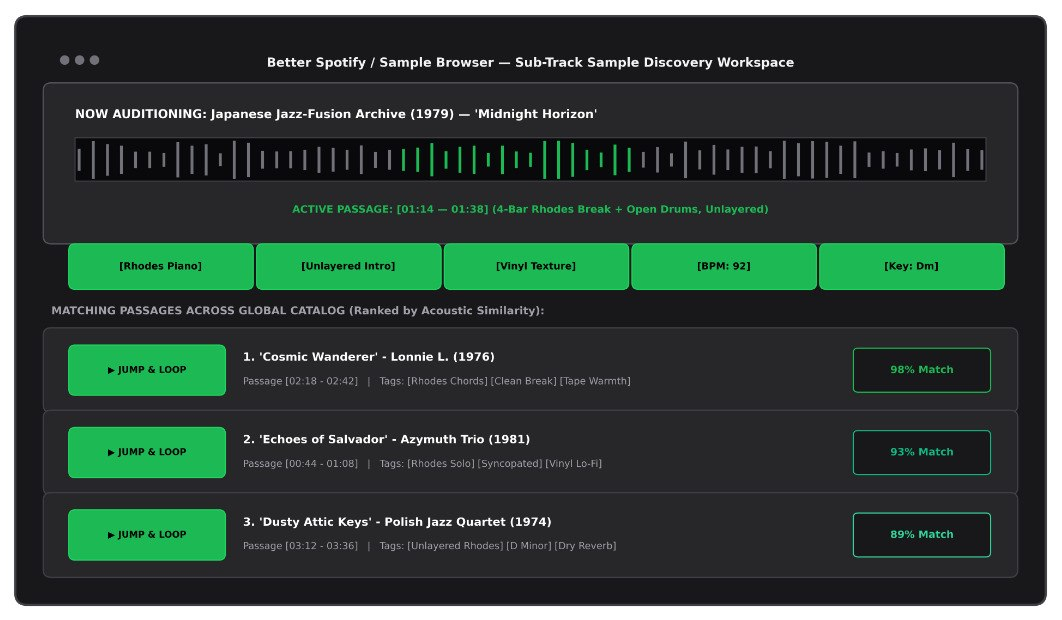
\includegraphics[width=\linewidth, height=3.8cm, keepaspectratio]{images/sample_browser_mockup.png}\par\vspace{1mm}
    {\tiny\textcolor{textdim}{Concept mockup (illustrative; match scores are not from a working algorithm)}}
  \end{tcolorbox}\par}

  \vspace{1.5mm}

  % Three Concise Capability Labels
  \begin{columns}[onlytextwidth, c]
    \begin{column}{0.315\textwidth}
      \begin{tcolorbox}[innercard, top=2.5pt, bottom=2.5pt]
        \centering
        {\scriptsize\bfseries\textcolor{accentemerald}{1. Acoustic Filters}}\par\vspace{0.2mm}
        {\tiny\textcolor{textmuted}{Instrument, texture, timbre}}
      \end{tcolorbox}
    \end{column}

    \begin{column}{0.315\textwidth}
      \begin{tcolorbox}[innercard, top=2.5pt, bottom=2.5pt]
        \centering
        {\scriptsize\bfseries\textcolor{accentemerald}{2. Passage Results}}\par\vspace{0.2mm}
        {\tiny\textcolor{textmuted}{Timestamped section candidates}}
      \end{tcolorbox}
    \end{column}

    \begin{column}{0.315\textwidth}
      \begin{tcolorbox}[innercard, top=2.5pt, bottom=2.5pt]
        \centering
        {\scriptsize\bfseries\textcolor{accentemerald}{3. Direct Cue + Loop}}\par\vspace{0.2mm}
        {\tiny\textcolor{textmuted}{Instant playhead jump (\texttt{seekTo})}}
      \end{tcolorbox}
    \end{column}
  \end{columns}
\end{frame}

\begin{frame}[t]
  \slideheader{05. SYSTEM ARCHITECTURE}{Interaction Pipeline \& Technical Scope}

  \begin{columns}[onlytextwidth, T]
    % Left Column: Architecture Diagram
    \begin{column}{0.54\textwidth}
      \begin{tcolorbox}[standardcard, top=3pt, bottom=3pt]
        \centering
        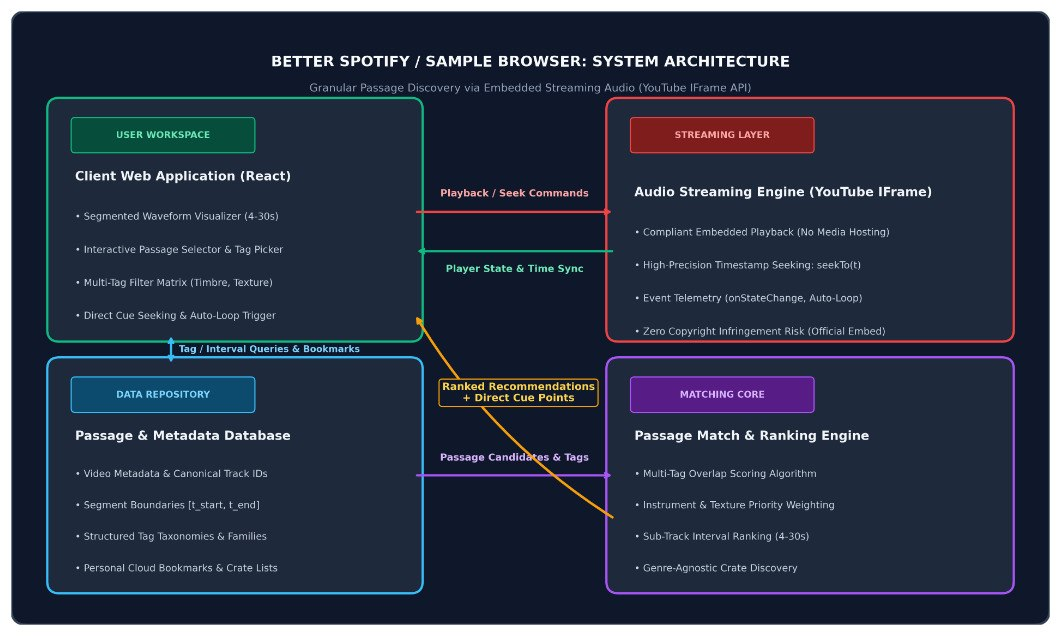
\includegraphics[width=\linewidth, height=3.4cm, keepaspectratio]{images/our_system_architecture.jpg}\par\vspace{0.8mm}
        {\tiny\textcolor{textdim}{\textbf{System Architecture:} Client UI, YouTube IFrame player, and PostgreSQL metadata backend.}}
      \end{tcolorbox}
    \end{column}

    % Right Column: Compact Pipeline & Technical Caveats
    \begin{column}{0.44\textwidth}
      % Interaction Pipeline
      \begin{tcolorbox}[standardcard, top=3.5pt, bottom=3.5pt]
        {\scriptsize\bfseries\textcolor{textwhite}{Interaction Pipeline}}\par\vspace{1.2mm}
        \centering
        {\tiny\textbf{\textcolor{textwhite}{Web UI}} \textcolor{textdim}{$\longrightarrow$} \textbf{\textcolor{textmuted}{Metadata}} \textcolor{textdim}{$\longrightarrow$} \textbf{\textcolor{textmuted}{Timestamp}} \textcolor{textdim}{$\longrightarrow$} \textbf{\textcolor{accentemerald}{YouTube Player}}}
      \end{tcolorbox}

      \vspace{1.5mm}

      % Implementation Scope
      \begin{tcolorbox}[standardcard, top=3.5pt, bottom=3.5pt]
        {\scriptsize\bfseries\textcolor{textwhite}{Implementation Status}}\par\vspace{1mm}
        {\tiny\textbf{\textcolor{textwhite}{Current:}} Curated acoustic tagging and timestamp metadata.}\\[0.8mm]
        {\tiny\textbf{\textcolor{accentemerald}{Planned (M2):}} Automated MIR indexing (Essentia classifiers).}\\[0.6mm]
        {\tiny\textcolor{textdim}{*Note: MIR indexing is planned for evaluation, not implemented.}}
      \end{tcolorbox}

      \vspace{1.5mm}

      % Honest Disclosure Caveat
      \begin{tcolorbox}[innercard, top=3pt, bottom=3pt]
        {\tiny\textcolor{textmuted}{\textbf{Technical Caveat:} Compliant audio ingestion for server-side MIR remains unresolved. No original audio hosting; user clears sampling rights.}}
      \end{tcolorbox}
    \end{column}
  \end{columns}
\end{frame}
\begin{frame}[t]
  \slideheader{06. COMPARATIVE ANALYSIS \& SWOT}{Competitive Positioning \& Strategic SWOT Overview}

  \begin{columns}[onlytextwidth, T]
    % Left Column: Competitive Positioning
    \begin{column}{0.485\textwidth}
      \begin{tcolorbox}[standardcard, top=3.5pt, bottom=3.5pt, left=6pt, right=6pt]
        {\scriptsize\bfseries\textcolor{textwhite}{Competitor Landscape}}\par\vspace{1.2mm}
        
        \begin{compactlist}
          \tiny
          \item \textbf{Splice:} Curated loop packs (isolated samples)
          \item \textbf{Samplette:} Whole-track YouTube discovery
          \item \textbf{Tracklib:} Pre-cleared catalog + looping tools
          \item \textbf{Sononym:} Local desktop similarity search
          \item \textbf{Cyanite:} Enterprise B2B sync intelligence
        \end{compactlist}

        \vspace{1.5mm}
        \begin{tcolorbox}[enhanced, colback=cardinner, colframe=accentemerald, boxrule=0.8pt, arc=3pt, top=3pt, bottom=3pt, left=5pt, right=5pt]
          {\tiny\textbf{\textcolor{accentemerald}{Proposed focus:}} \textcolor{textwhite}{a creator workflow combining acoustic filters, passage-level search across recordings, and direct timestamp auditioning.}}
        \end{tcolorbox}
      \end{tcolorbox}
    \end{column}

    % Right Column: Balanced 2x2 SWOT Grid
    \begin{column}{0.485\textwidth}
      \begin{tcolorbox}[standardcard, top=3.5pt, bottom=3.5pt, left=6pt, right=6pt]
        {\scriptsize\bfseries\textcolor{textwhite}{Strategic SWOT Overview}}\par\vspace{1.2mm}
        
        \begin{columns}[onlytextwidth, T]
          % Strengths
          \begin{column}{0.48\textwidth}
            \begin{tcolorbox}[innercard, top=3pt, bottom=3pt, left=3.5pt, right=3.5pt]
              {\scriptsize\bfseries\textcolor{accentemerald}{Strengths (S)}}\par\vspace{0.6mm}
              {\tiny\textbullet{} Sub-track granularity}\\[0.2mm]
              {\tiny\textbullet{} Direct timestamp cueing}\\[0.2mm]
              {\tiny\textbullet{} No original audio hosting}
            \end{tcolorbox}
          \end{column}
          % Weaknesses
          \begin{column}{0.48\textwidth}
            \begin{tcolorbox}[innercard, top=3pt, bottom=3pt, left=3.5pt, right=3.5pt]
              {\scriptsize\bfseries\textcolor{textdim}{Weaknesses (W)}}\par\vspace{0.6mm}
              {\tiny\textbullet{} Cold-start catalog}\\[0.2mm]
              {\tiny\textbullet{} Stream dependency}\\[0.2mm]
              {\tiny\textbullet{} Unresolved MIR ingest}
            \end{tcolorbox}
          \end{column}
        \end{columns}

        \vspace{1mm}

        \begin{columns}[onlytextwidth, T]
          % Opportunities
          \begin{column}{0.48\textwidth}
            \begin{tcolorbox}[innercard, top=3pt, bottom=3pt, left=3.5pt, right=3.5pt]
              {\scriptsize\bfseries\textcolor{accentemerald}{Opportunities (O)}}\par\vspace{0.6mm}
              {\tiny\textbullet{} Sample pack fatigue}\\[0.2mm]
              {\tiny\textbullet{} Future DAW integration}\\[0.2mm]
              {\tiny\textbullet{} Label partnerships}
            \end{tcolorbox}
          \end{column}
          % Threats
          \begin{column}{0.48\textwidth}
            \begin{tcolorbox}[innercard, top=3pt, bottom=3pt, left=3.5pt, right=3.5pt]
              {\scriptsize\bfseries\textcolor{textdim}{Threats (T)}}\par\vspace{0.6mm}
              {\tiny\textbullet{} Streaming API shifts}\\[0.2mm]
              {\tiny\textbullet{} Incumbent feature creep}\\[0.2mm]
              {\tiny\textbullet{} Clearance friction}
            \end{tcolorbox}
          \end{column}
        \end{columns}
      \end{tcolorbox}
    \end{column}
  \end{columns}

  \vspace{1.5mm}

  % Bottom Note
  \begin{tcolorbox}[innercard, left=6pt, right=6pt, top=2pt, bottom=2pt]
    \centering
    {\tiny\textcolor{textdim}{*Full comparative matrix and complete SWOT analysis preserved in} \textbf{\textcolor{accentemerald}{Appendix (Slides 10--11)}} \textcolor{textdim}{for committee Q\&A.}}
  \end{tcolorbox}
\end{frame}

\begin{frame}[t]
  \slideheader{07. CUSTOMER VALIDATION, BUSINESS MODEL \& ROADMAP}{Engineering Roadmap \& Validation Hypotheses}

  % Dominant Visual: Enlarged 3-Stage Horizontal Roadmap
  \begin{columns}[onlytextwidth, T]
    % Stage 1: Validate
    \begin{column}{0.315\textwidth}
      \begin{tcolorbox}[standardcard, top=3.5pt, bottom=3.5pt, left=5pt, right=5pt]
        {\normalsize\bfseries\textcolor{accentemerald}{1. Validate}}\\[0.4mm]
        {\scriptsize\bfseries\textcolor{textwhite}{10--15 Producer Interviews}}\par\vspace{0.8mm}
        {\tiny\textcolor{textmuted}{Direct interviews on workflow friction and digging habits.}}
      \end{tcolorbox}
    \end{column}

    % Stage 2: Prototype
    \begin{column}{0.315\textwidth}
      \begin{tcolorbox}[standardcard, top=3.5pt, bottom=3.5pt, left=5pt, right=5pt]
        {\normalsize\bfseries\textcolor{textwhite}{2. Prototype (M2)}}\\[0.4mm]
        {\scriptsize\bfseries\textcolor{textwhite}{Interactive UI \& Architecture}}\par\vspace{0.8mm}
        {\tiny\textcolor{textmuted}{Functional wireframing and UML structural models.}}
      \end{tcolorbox}
    \end{column}

    % Stage 3: Evaluate
    \begin{column}{0.315\textwidth}
      \begin{tcolorbox}[standardcard, top=3.5pt, bottom=3.5pt, left=5pt, right=5pt]
        {\normalsize\bfseries\textcolor{textwhite}{3. Evaluate (Exam)}}\\[0.4mm]
        {\scriptsize\bfseries\textcolor{textwhite}{Passage Utility Assessment}}\par\vspace{0.8mm}
        {\tiny\textcolor{textmuted}{Empirical evaluation of passage retrieval utility.}}
      \end{tcolorbox}
    \end{column}
  \end{columns}

  \vspace{1.2mm}

  % Middle Row: Hypotheses Tags & Business Model
  \begin{columns}[onlytextwidth, T]
    % Left: Research Direction Tags
    \begin{column}{0.485\textwidth}
      \begin{tcolorbox}[innercard, top=2.5pt, bottom=2.5pt, left=5pt, right=5pt]
        {\scriptsize\bfseries\textcolor{textwhite}{Research Hypotheses (To Investigate):}}\par\vspace{0.8mm}
        \centering
        {\scriptsize\textbf{\textcolor{accentemerald}{[Scrubbing Pain (H1)]}} \quad \textbf{\textcolor{textwhite}{[Tool Gap (H2)]}} \quad \textbf{\textcolor{accentemerald}{[Time Target (H3)]}}}\par\vspace{0.8mm}
        {\tiny\textcolor{textdim}{Field validation planned across $N=10\text{--}15$ creator interviews}}
      \end{tcolorbox}
    \end{column}

    % Right: Potential Business Model
    \begin{column}{0.485\textwidth}
      \begin{tcolorbox}[innercard, top=2.5pt, bottom=2.5pt, left=5pt, right=5pt]
        {\scriptsize\bfseries\textcolor{textwhite}{Potential Business Model (To Be Validated):}}\par\vspace{0.6mm}
        \centering
        {\scriptsize\textbf{\textcolor{textwhite}{Free Community Tier}} \quad \textbar \quad \textbf{\textcolor{accentemerald}{Pro Creator Tier}}}\par\vspace{0.4mm}
        {\tiny\textcolor{textmuted}{\textbf{Pro Tier (hypothesis):} Timbral MIR similarity, DAW marker exports (MIDI/cue), unlimited crates}}\par\vspace{0.2mm}
        {\tiny\textcolor{textdim}{*Monetization viability remains an unvalidated hypothesis.}}
      \end{tcolorbox}
    \end{column}
  \end{columns}

  \vspace{1.2mm}

  % Bottom Final Takeaway Banner
  \begin{tcolorbox}[standardcard, left=6pt, right=6pt, top=2.5pt, bottom=2.5pt]
    \centering
    {\small\textbf{\textcolor{accentemerald}{Takeaway:}} \textcolor{textwhite}{Sample Browser explores a missing link between finding a recording and finding the exact passage worth using.}}
  \end{tcolorbox}
\end{frame}


\appendix
\begin{frame}[t]
  \slideheader{APPENDIX · Q\&A REFERENCE}{Strategic SWOT Analysis (Report Section 2.4, Table 3)}

  % 2x2 Grid of Editable LaTeX Cards
  \begin{columns}[onlytextwidth, T]
    % Quadrant 1: Strengths
    \begin{column}{0.485\textwidth}
      \begin{tcolorbox}[standardcard, top=3pt, bottom=3pt]
        {\scriptsize\bfseries\textcolor{accentemerald}{STRENGTHS (S)}}\par\vspace{0.8mm}
        \begin{compactlist}
          \tiny
          \item \textbf{Sub-Track Granularity:} Indexes at 2--16 bar interval level, designed to reduce manual scrubbing.
          \item \textbf{Explainable Discovery:} Transparent acoustic descriptors rather than opaque black-box recommendations.
          \item \textbf{No Original Audio Hosting:} Uses compliant YouTube IFrame streaming without media storage overhead.
          \item \textbf{Contextual Playback:} Audition passages in original arrangements.
        \end{compactlist}
      \end{tcolorbox}
    \end{column}

    % Quadrant 2: Weaknesses
    \begin{column}{0.485\textwidth}
      \begin{tcolorbox}[standardcard, top=3pt, bottom=3pt]
        {\scriptsize\bfseries\textcolor{textdim}{WEAKNESSES (W)}}\par\vspace{0.8mm}
        \begin{compactlist}
          \tiny
          \item \textbf{Cold-Start Catalog Challenge:} Platform utility in early stages relies heavily on pre-tagged passage volume.
          \item \textbf{Third-Party Dependency:} Vulnerable to YouTube video takedowns, regional geo-blocks, or API policy changes.
          \item \textbf{No Direct Audio Export:} Users must acquire source audio externally under API terms.
        \end{compactlist}
      \end{tcolorbox}
    \end{column}
  \end{columns}

  \vspace{1.5mm}

  \begin{columns}[onlytextwidth, T]
    % Quadrant 3: Opportunities
    \begin{column}{0.485\textwidth}
      \begin{tcolorbox}[standardcard, top=3pt, bottom=3pt]
        {\scriptsize\bfseries\textcolor{accentemerald}{OPPORTUNITIES (O)}}\par\vspace{0.8mm}
        \begin{compactlist}
          \tiny
          \item \textbf{Sample Pack Fatigue:} Producer backlash against overused commercial sample libraries (Splice).
          \item \textbf{DAW Plugin Integration:} Potential to port interface into embedded VST/AU inside Ableton or FL Studio.
          \item \textbf{Catalog Rights Monetization:} Partnership pathways with archival labels to monetize dormant back-catalogs.
        \end{compactlist}
      \end{tcolorbox}
    \end{column}

    % Quadrant 4: Threats
    \begin{column}{0.485\textwidth}
      \begin{tcolorbox}[standardcard, top=3pt, bottom=3pt]
        {\scriptsize\bfseries\textcolor{textdim}{THREATS (T)}}\par\vspace{0.8mm}
        \begin{compactlist}
          \tiny
          \item \textbf{API Policy Lockdowns:} Risk of streaming providers restricting embedded player functionality.
          \item \textbf{Incumbent Expansion:} Established tools (Tracklib, Samplette) expanding into segment-level tagging.
          \item \textbf{Copyright Uncertainties:} Legal clearance requirements for archival recordings in commercial releases.
        \end{compactlist}
      \end{tcolorbox}
    \end{column}
  \end{columns}
\end{frame}

\begin{frame}[t]
  \slideheader{APPENDIX · Q\&A REFERENCE}{Formal Problem Statement \& Evaluation Matrix}

  % Formal Problem Statement Card
  \begin{tcolorbox}[standardcard, top=3pt, bottom=3pt]
    {\tiny\bfseries\textcolor{accentemerald}{VERBATIM FORMAL PROBLEM STATEMENT (REPORT SEC. 2.1)}}\par\vspace{0.6mm}
    {\scriptsize\itshape\textcolor{textwhite}{"Independent music producers lack an efficient way to discover and locate specific musical passages within full-length catalog recordings based on acoustic references, because contemporary streaming search interfaces index music exclusively at the whole-track metadata level, forcing producers into tedious, manual scrubbing that disrupts the creative workflow."}}
  \end{tcolorbox}

  \vspace{1.5mm}

  % Comparative Evaluation Matrix (Table 2)
  \begin{tcolorbox}[standardcard, top=3pt, bottom=3pt]
    {\scriptsize\bfseries\textcolor{textwhite}{Comparative Tool Matrix (Report Table 2)}}\par\vspace{1mm}
    \tiny
    \begin{tabularx}{\textwidth}{@{}l l l l X@{}}
      \toprule
      \textbf{Platform} & \textbf{Index Granularity} & \textbf{Query Paradigm} & \textbf{Catalog Type} & \textbf{Workflow Role} \\
      \midrule
      \textbf{Splice} & Isolated samples & Text / Metadata & Curated proprietary & Ready-made sound packs \\
      \textbf{Samplette} & Full-track & Random / Discogs & Public (YouTube) & Full-record digging \\
      \textbf{Tracklib} & Track + Bar loops & Metadata / Mood & Pre-cleared master & Licensing marketplace \\
      \textbf{Sononym} & Local sample files & Audio similarity & Local user disk & Sample library organizer \\
      \textbf{Cyanite.ai} & Track \& Segment & Audio similarity & Enterprise B2B & Sync intelligence API \\
      \midrule
      \textbf{\textcolor{accentemerald}{Sample Browser}} & \textbf{\textcolor{accentemerald}{Passage (4--30s)}} & \textbf{\textcolor{accentemerald}{Acoustic descriptors}} & \textbf{\textcolor{accentemerald}{Public (YouTube)}} & \textbf{\textcolor{accentemerald}{Cross-catalog discovery}} \\
      \bottomrule
    \end{tabularx}
  \end{tcolorbox}
\end{frame}


\end{document}
